\mbchapter{Aufbau einer Testanwendung}

In den folgenden Kapiteln werden Implementierungen für verschiedene Anwendungsszenarien beschrieben und verglichen. All diese verschiedenen Implementierungen sollen in einer einzigen App zusammengefasst werden, um sie dadurch leicht auf verschiedenen Geräten testen zu können. Aus diesem Grund wird in diesem Abschnitt eine App beschrieben, die Modular aufgebaut ist und es ermöglicht, alle Implementierungen in einer App zu integrieren. Im Folgenden wird jeder Implementierungsansatz als Modul bezeichnet. Die App basiert grundsätzlich auf den gleichen Technologien und Frameworks, die in dieser Arbeit betrachtet werden. Zusätzlich wird neben der bereits beschriebene Library BenchmarkJS, die Library LoDash\footnote{https://lodash.com/} verwendet. LoDash enthält viele Funktionen für die Interaktion mit Arrays und Objekten.
\\\\
Um die Navigation zu vereinfachen folgt die Oberfläche der App einem Master-Detail Ansatz. Nach dem Start wird dem Anwender eine Liste aller Module angezeigt. Jedes Modul dieser Liste besitzt einen eindeutigen Namen und verweist auf eine Seite, die den Test für das jeweilige Modul beinhaltet. Die Seiten der einzelnen Module werden individuell und dem Test entsprechend gestaltet. Über einen Button in der linken oberen Ecke kann der Anwender zurück zur Liste der Module navigieren. Thematisch zusammenhängende Module werden über eine Kodierung im Namen gruppiert.  
\begin{figure}
	\centering
	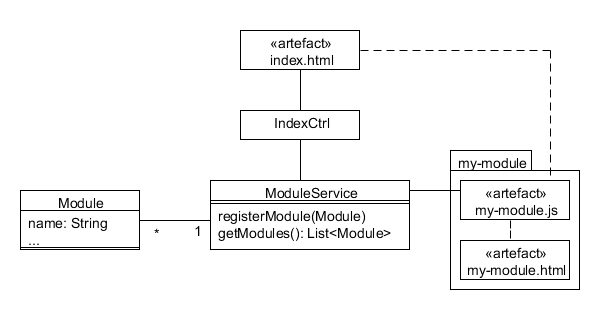
\includegraphics[scale=0.6]{Bilder/Testanwendung.png}
	\caption{Struktur der Testanwendung}
	\label{struktur-testanwendung}
\end{figure}
Um die Ergebnisse eines Tests nicht zu beeinflussen, müssen Tests isoliert von einander ausgeführt werden. Dies setzt voraus, dass die einzelnen Module untereinander keine und mit der App möglichst wenige Schnittpunkte besitzen. Außerdem ist es einfacher neue Module hinzuzufügen, wenn die App an sich nicht geändert werden muss. Damit die App diesen Anforderungen genügt, werden Module in einem Unterordner der Anwendung abgelegt. Jedes Modul besteht mindestens aus einer JavaScript-Datei und einer \gls{html}-Datei. Die JavaScript-Datei muss in der App als Skript referenziert werden (\emph{index.html}). Dies ist der einzige Eingriff in die Implementierung der App. In der JavaScript-Datei wird das Modul in einem globalen Service registriert und dabei einem Zustandsgraphen für das \gls{Routing} in der Anwendung hinzugefügt. Beim Start der Anwendung ruft die App alle registrierten Module von diesem globalen Service ab und zeigt sie mit ihrem Namen in der Liste an. Klickt der Anwender auf ein Modul, wechselt die App über den \gls{Routing}-Mechanismus zu dessen \gls{html}-Datei. Dort werden Interaktionen und Informationen für den jeweilige Test angezeigt. Für das Erstellen neuer Module reicht es demnach aus, die beiden Dateien anzulegen, in der \emph{index.html} zu referenzieren und per JavaScript zu registrieren. Module haben keine implizite Verknüpfung untereinander oder mit der Anwendung und werden daher grundsätzlich isoliert voneinander ausgeführt. Um weitere Seiteneffekte zu vermeiden, werden in der App sämtliche von AngularJS durchgeführte Optimierungen und Animationen ausgeschaltet. Dazu zählt das Zwischenspeichern bereits besuchter Seiten, sowie das vorzeitige Laden von Templates.